\begin{figure*}
  \centering
  % \begin{noindent}
  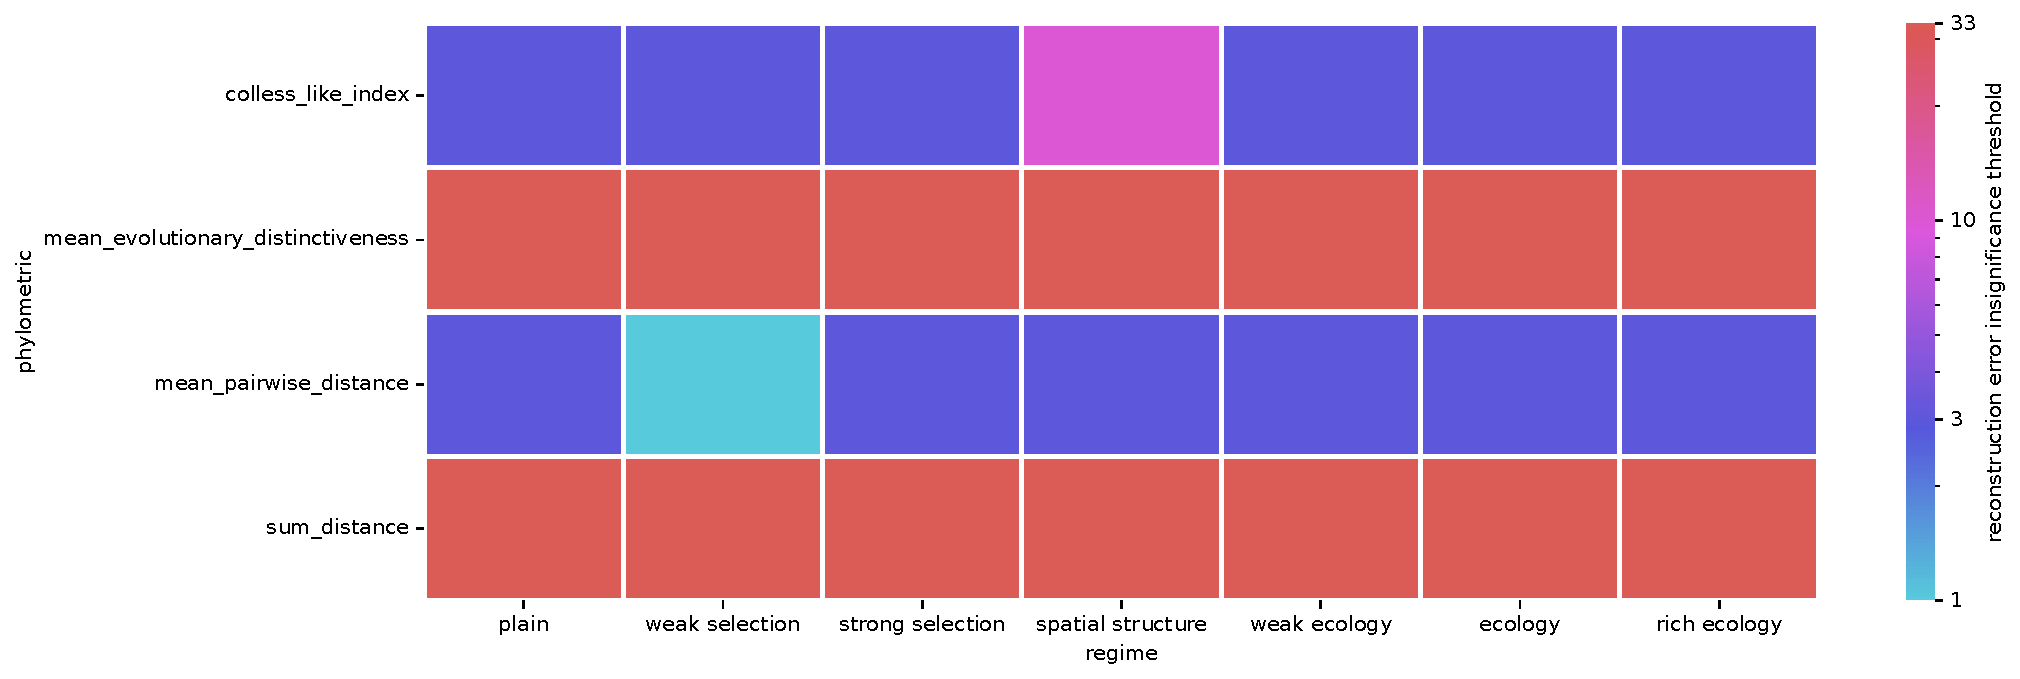
\includegraphics[width=\textwidth]{binder/binder/teeplots/epoch=7+hue=quality-threshold+mut_distn=np.random.standard_normal+viz=heatmap+x=regime+y=phylometric+ext=.pdf}
  % \end{noindent}
  \caption{%
    \textbf{Reconstruction resolutions required to achieve statistical indistinguishability between reconstructions and ground-truth reference trees.}
    Significance level $p<0.05$ under the Wilcoxon signed-rank test between samples of 50 replicates each is used as the threshold for statistical distinguishability.
    Phylometrics with looser reconstruction resolution thresholds (i.e., higher resolution percentages) are less sensitive to reconstruction error.
    White heat map tiles indicate that no surveyed reconstruction resolution threshold was sufficient to achieve indistinguishability from the reference tree with respect a particular phylometric.
    See Supplementary Figure \ref{fig:reconstructed-tree-phylometrics-error-sensitivity-analysis} for sensitivity analysis results.
  }
  \label{fig:reconstructed-tree-phylometrics-error}
\end{figure*}
